% !TEX root = ../../I4PRJ, Grp3 - Rapport.tex
\chapter{Arkitektur}
I dette afsnit beskrives den overordnede arkitektur for systemet. Systemets arkitektur har dannet ramme for design og senere implementering. Domæneanalyse giver anledning til en 3-tier arkitektur, da systemet har tre domæner, som er application, server og database.

\section{3 Tier Model}

I det følgende vil de tre tiers blive beskrevet.

\begin{figure}
	\centering
	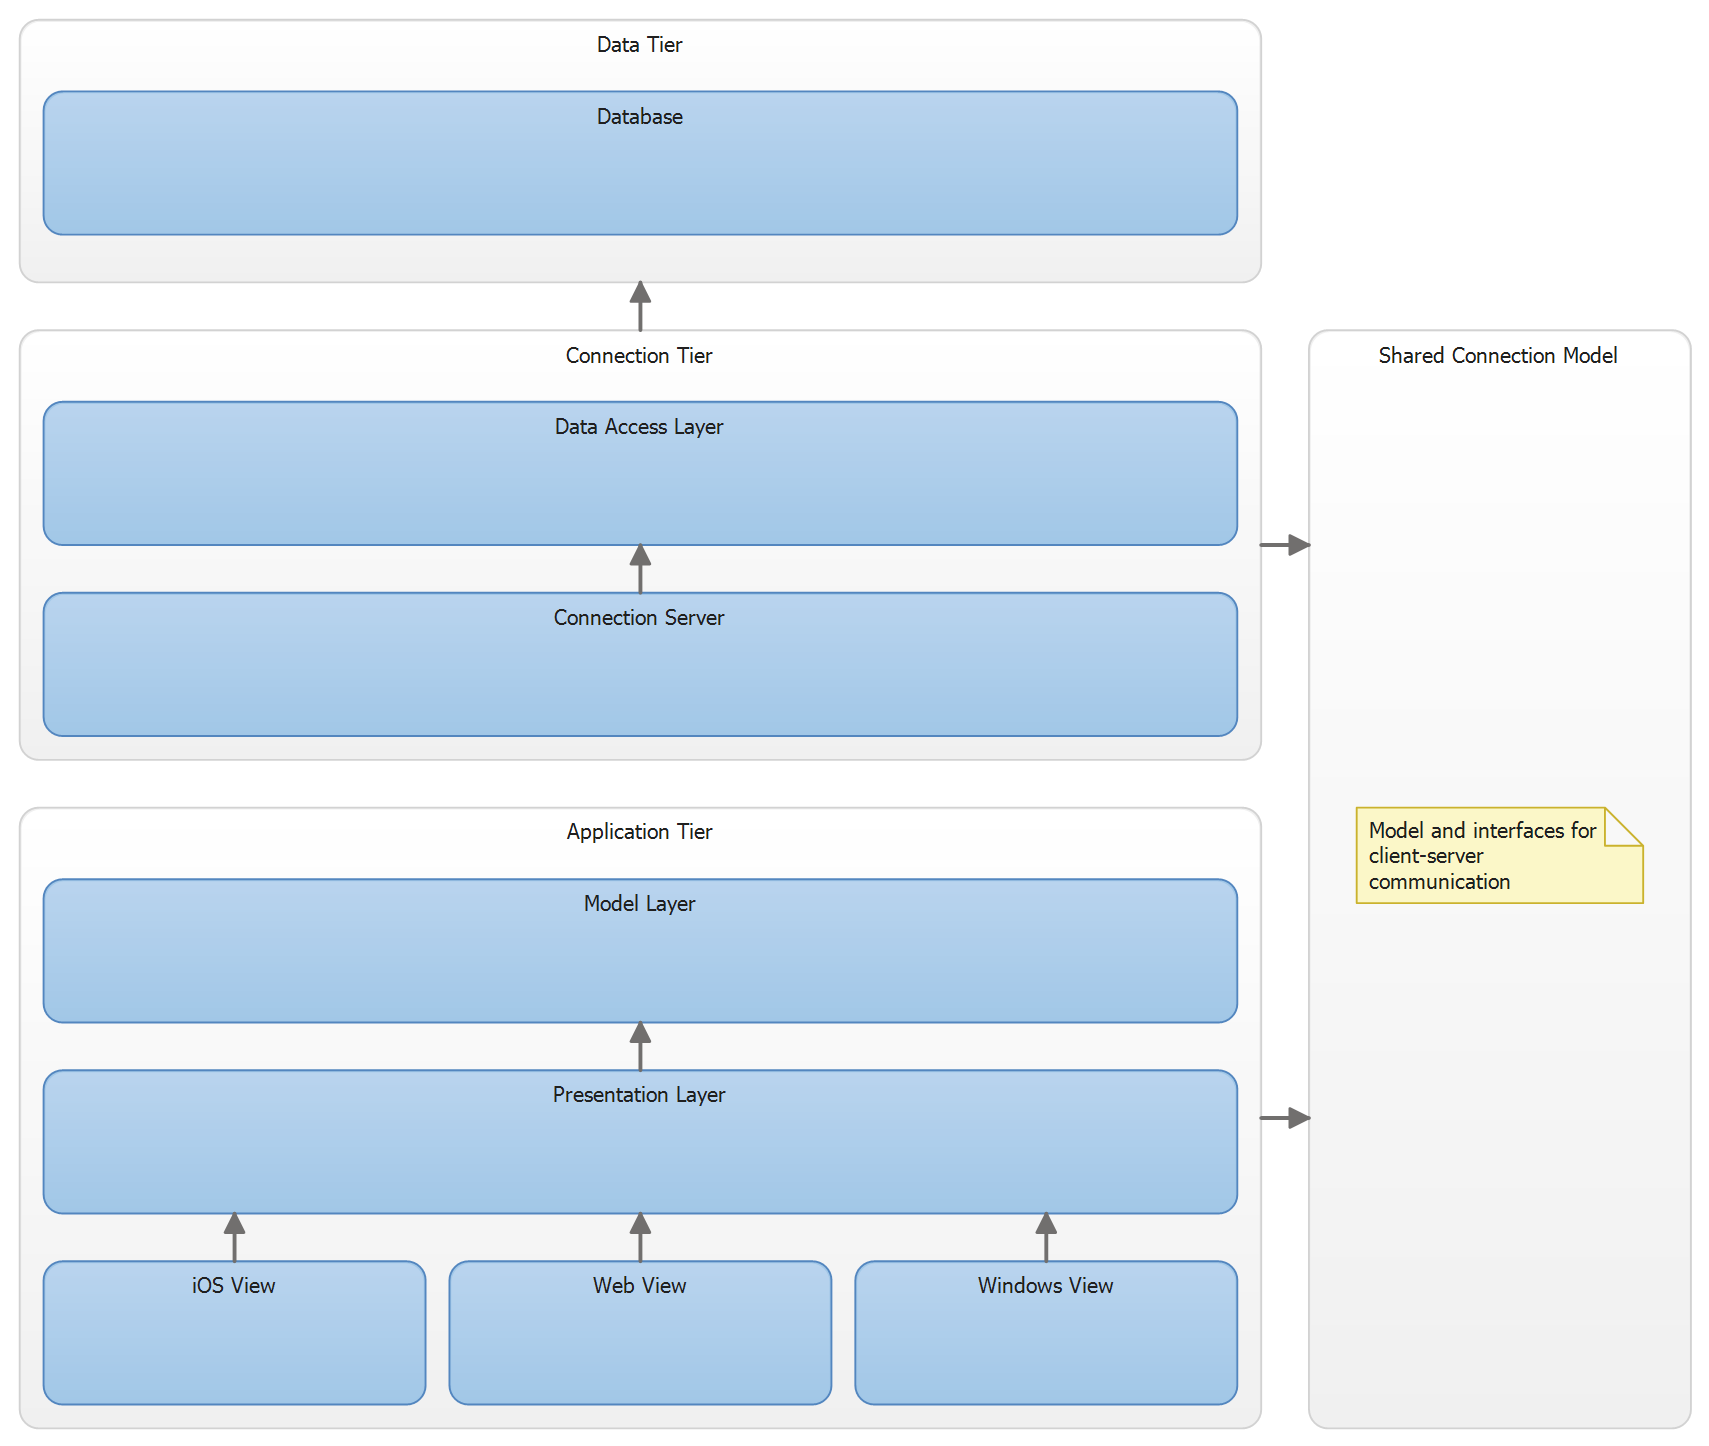
\includegraphics[width=\linewidth]{figs/arkitektur/Smartpool_tiersnlayers}
	\caption{Tiers and layers}
	\label{fig:tiersnlayers}
\end{figure}

\subsection{Application Tier}
Det ønskes at afkoble view fra præsentationslogikken og modellen. Til det formål benyttes GUI arkitekturen MVP. Det bruges så viewet er afkoblet og dermed kan udskiftes. Det er gjort med henblik på, at genbruge præsentationslogikken på flere platforme. Application tier kommunikerer med Connection tier igennem en Shared Connection Model jf. figur~\ref{fig:tiersnlayers}. 

\subsection{Connection Tier}\label{sec:Connectiontier}
Da det ønskes at adskille systemets business logic fra brugerens applikation, er der oprettet en server som står for dette. Da systemets primære opgave er at gemme og vise data, består dette primært i at lave kald til databasen. Ved at have disse kald i en separat server applikation, sikrer vi at brugerens adgang til databasen, kun går gennem serveren, som dermed kan beskytte de kritiske data.

\subsection{Data Tier}
Data-access laget er sammen med \gls{windserver} afkoblet fra Applikations tier'et. Dette betyder at forbindelsen til databasen, sker fra Applikations tier'et gennem \gls{windserver}. Data-access laget som er designet med Entity Frameworket, kommunikerer da med selve databasen.
\section{4+1 Arkitektur Model}
Systemets arkitektur er beskrevet ved 4+1 modellen. 4+1 modellen består af en række views, som hver især henvender sig til forskellige interessenter.

\subsection{Logical view}
Logical view beskriver funktionaliteten for systemets end-user. Logical view repræsenteres ved et Activity diagram. Figur~\ref{fig:ActivityDiagram} illustrerer et typisk brugsscenarie for en end-user. 
\begin{figure}
\centering
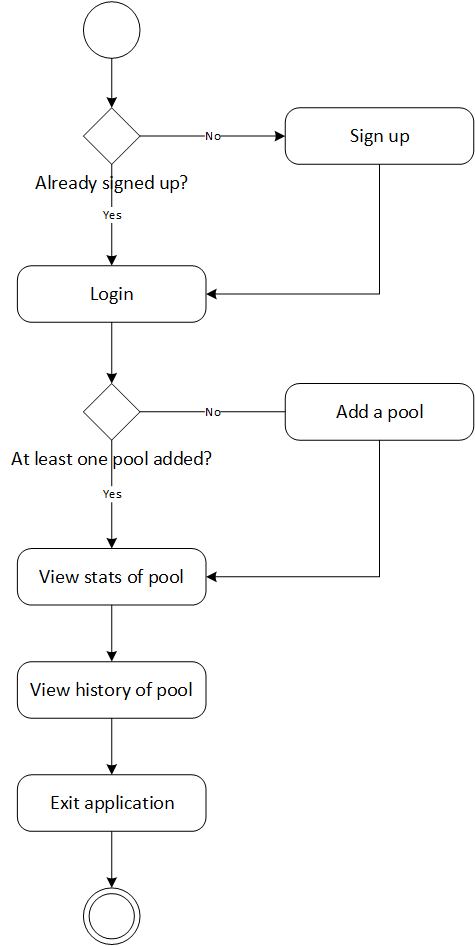
\includegraphics[width=0.55\linewidth]{figs/arkitektur/ActivityDiagram.PNG}
\caption{Activity diagram}
\label{fig:ActivityDiagram}
\end{figure}

De andre views for systemet forefindes i dokumentationen, da disse henvender sig primært til udviklere.
